As we've recounted the axioms of AQFT in Minkowski spacetime, we are now in a position to generalize this to curved spacetime, i.e. ``Lorentzian spacetime''. Surprisingly the generalization to ``Lorentzian spacetime'' is relatively straightforward.

We note, however, that as in the case of AQFT in Minkowski spacetime, the generalization to ``Lorentzian spacetime'' will not account for ``backreaction'' of the quantum fields on ``Lorentzian spacetime''. The ``Lorentzian spacetime'' will be a fixed, classical background upon which AQFT ``unfolds''.

\section{Prologue}\label{sctn:prologue}
Most presentations of AQFT in curved spacetime gloss over the details of exactly what ``Lorentzian spacetime'' is. It's too ``basic''.

In contrast to those presentations, we want to spend some time detailing exactly what ``Lorentzian spacetime'' is before we formulate AQFT there. This level of pedantry will serve us well when formulating AQFT on ``Lorentzian spacetime'', helping to motivate otherwise opaque aspects of the formulation.

\subsection{Smooth Manifold}
Consider a smooth, connected, four dimensional Hausdorff manifold $M$ equipped with a topology, which we simply call the ``manifold topology''. This will form the ``core'' of our definition of a ``Lorentzian spacetime''.

\subsection{Existence of a Lorentzian Metric}
As we wish this $M$ to be a ``Lorentzian spacetime'', it should support a Lorentzian metric. Not all such $M$ support Lorentzian metrics. In fact for such an $M$ to support a Lorentzian metric, it must admit additional structure.

In particular, as we have seen previously, the required structure follows from the theorem (Theorem 2.69 from \href{https://doi.org/10.1007/978-3-319-91755-9}{Lee})

\begin{theorem}[Existence of a Lorentz Metric]
    A smooth manifold $M$ admits a smooth Lorentz metric if and only if it admits a smooth, nowhere-vanishing global vector field.
\end{theorem}

So, we require, in addition to all the structure $M$ already supports, that it also supports a smooth, nowhere-vanishing global vector field $t^a$, as this is required for $M$ to support a smooth Lorentzian metric.

\subsection{Alexandrov Topology}
As in the case of a Minkowski spacetime, it's ``odd'' that the manifold topology on $M$ may have nothing to do with the Lorentzian nature of spacetime. The manifold topology could, as was the case for Minkowski spacetime, be derived from purely Euclidean metrics. Physics isn't Euclidean; so there seems to be a fundamental tension.

In the case of Minkowski spacetime we introduced sets of the form $I^+(p) \cap I^-(q)$, showed that they are open in the Euclidean topology (Proposition 2.8 of \href{https://doi.org/10.1137/1.9781611970609}{Penrose}), and can be used as the basis of the Alexandrov topology (Definition 4.22 of \href{https://doi.org/10.1137/1.9781611970609}{Penrose}). Furthermore, we showed that the Alexandrov topology is equivalent to the Euclidean topology (Paragraph 4.23 of \href{https://doi.org/10.1137/1.9781611970609}{Penrose}). We want to generalize all of this to ``Lorentzian spacetimes''.

It turns out that just as in the case of Minkowski spacetime, sets of the form $I^+(p) \cap I^-(q)$ on $M$ are open sets in the manifold topology (Proposition 2.8 of \href{https://doi.org/10.1137/1.9781611970609}{Penrose}). Furthermore, on $M$ they also form the basis of a topology (Definition 4.22 of \href{https://doi.org/10.1137/1.9781611970609}{Penrose}), again called the Alexandrov topology. However, for $M$ the relationship between the Alexandrov topology and the manifold topology is more nuanced than in the case of Minkowski spacetime.

It turns out that to understand this nuance, we need to introduce several definitions that aid in the process.

\begin{definition}[Causally Convex]
    Consider an open subset $\mathbf{O}$ of a smooth, connected, four dimensional Hausdorff manifold $M$ that is equipped with a Lorentzian metric. $\mathbf{O}$ is said to be \textit{causally convex} if for every $p$ and $r$ in $\mathbf{O}$ and $q$ in $M$ the existence of a future-directed, time-like curve from $p$ to $q$ and a future-directed, time-like curve from $q$ to $r$ implies that $q$ is a member of $\mathbf{O}$.
\end{definition}

\begin{definition}[Strongly Causal]
    Consider a smooth, connected, four dimensional Hausdorff manifold $M$ that is equipped with a Lorentzian metric. $M$ is said to be \textit{strongly causal} at $p \in M$ if $p$ has arbitrarily small causally convex neighborhoods. $M$ is said to be \textit{strongly causal} if $M$ is strongly causal at every $p \in M$.
\end{definition}

With these definitions in hand we can then present the key theorem describing how the Alexandrov topology and the manifold topology are related (Theorem 4.24 of \href{https://doi.org/10.1137/1.9781611970609}{Penrose}):

\begin{theorem}[Properties of the Alexandrov Topology]
    The following three conditions on a smooth, connected, four dimensional manifold $M$ with Hausdorff manifold topology are equivalent:
    \begin{enumerate}
        \item $M$ is strongly causal;
        \item the Alexandrov Topology agrees with the manifold topology;
        \item the Alexandrov Topology is Hausdorff.
    \end{enumerate}
\end{theorem}

As one can see, this has ``deep'' implications for the case at hand, the smooth manifold $M$.

Physically, the Alexandrov topology seems more ``natural'' as it relies upon basis elements $I^+(p) \cap I^-(q)$ ``natural'' to Lorentzian nature of spacetime. So physically one would expect a ``Lorentzian spacetime'' to ``naturally'' be equipped with an Alexandrov topology. The question is how does one accomplish this goal?

In the case of Minkowski spacetime the Alexandrov topology on $\mathbb{R}^4$ agreed with the Euclidean topology without any further assumptions. The Euclidean ``scaffolding'' used to construct the Alexandrov topology simply ``fell away''. The previous theorem implies that for the more general case we are dealing with now on $M$, removing the manifold topology ``scaffolding'' requires additional assumptions.

In particular, we can either assume that $M$ is strongly causal or that the Alexandrov Topology is Hausdorff. Either assumption implies the other and that the Alexandrov Topology agrees with the manifold topology, and thus the manifold topology ``scaffolding'' can be removed.

As both assumptions are equivalent, we can select either. With that in mind, we add the additional assumption that the Alexandrov Topology on $M$ is Hausdorff. So in total $M$ is a smooth, connected, four dimensional manifold equipped with a smooth, nowhere-vanishing global vector field $t^a$ and associated Lorentzian metric. In addition $M$ is equipped with an associated Hausdorff Alexandrov Topology.

\subsection{Lorentzian Spacetime}
Finally we have all the pieces in place to define a ``Lorentzian spacetime''.

\begin{definition}[Lorentzian Spacetime]
    A \textit{Lorentzian spacetime} is a smooth, connected, four dimensional manifold equipped with a smooth, nowhere-vanishing global vector field $t^a$ and associated Lorentzian metric. In addition it is equipped with an associated Hausdorff Alexandrov topology.
\end{definition}

It will be on such Lorentzian spacetimes that AQFT ``unfolds''.


\section{Axiom 1 (Local Algebras)}\label{sctn:axiom-1-(local-algebras)}
With the prologue complete, we are now in a position to state the axioms of AQFT on Lorentzian spacetime. Surprisingly, all the hard work is done.

The first axiom is:

\begin{axiom}[Local Algebras]
    For any basis element $\mathbf{B}$ of the Alexandrov topology on a Lorentzian spacetime, i.e. any set of the form $I^+(p) \cap I^-(q)$, there is a corresponding abstract C*-algebra $\mathfrak{U}(\mathbf{B})$
    \begin{align}
        \mathbf{B} \longmapsto \mathfrak{U}(\mathbf{B}),
    \end{align}
    and when $\mathbf{B}$ is the empty set, we have the distinguished correspondence
    \begin{align}
        \emptyset \longmapsto \mathbb{C} \mathbf{1},
    \end{align}
    where $\mathbf{1}$ is the multiplicative identity in the abstract C*-algebra $\mathbb{C} \mathbf{1}$.
\end{axiom}


\section{Axiom 2 (Isotony)}\label{sctn:axiom-2-(isotony)}
The second axiom takes the following form:

\begin{axiom}[Isotony]
    Let $\mathbf{B}_1$ and $\mathbf{B}_2$ be any two basis elements of the Alexandrov topology on a Lorentzian spacetime, i.e. any two sets of the form $I^+(p_1) \cap I^-(q_1)$ and $I^+(p_2) \cap I^-(q_2)$.
    
    If $\mathbf{B}_1 \subset \mathbf{B}_2$ then $\mathfrak{U}(\mathbf{B}_1) \subset \mathfrak{U}(\mathbf{B}_2)$, where inclusion is implemented by
    \begin{align}
        i : \mathfrak{U}(\mathbf{B}_1) \hookrightarrow \mathfrak{U}(\mathbf{B}_2),
    \end{align}
    a unital *-monomorphism.
\end{axiom}


\section{Axiom 3 (Local Commutativity)}\label{sctn:axiom-3-(local-commutativity)}
So far the axioms have differed little from those of AQFT in Minkowski spacetime. This ceases to be true for subsequent axioms. The primary reason for this is that the existence of a quasilocal algebra is not guaranteed on a Lorentzian spacetime. Let us prove this is the case.

\subsection{Quasilocal Algebra?}
Naively, to define a quasilocal algebra associated with a Lorentzian spacetime $M$ one would first consider the set-theoretic union of all $\mathfrak{U}(\mathbf{B})$ over all basis elements $\mathbf{B}$ of the Alexandrov topology on $M$ and prove this set-theoretic union is a normed *-algebra. It turns out that for a generic Lorentzian spacetime $M$ this set-theoretic union isn't a normed *-algebra and thus the construction of the quasilocal algebra fails. Let's see why this is the case.

Consider $M_{BH}$ the Schwarzschild blackhole solution Lorentzian spacetime. $M_{BH}$ has the following Penrose diagram
\begin{figure}[h]
    \centering
    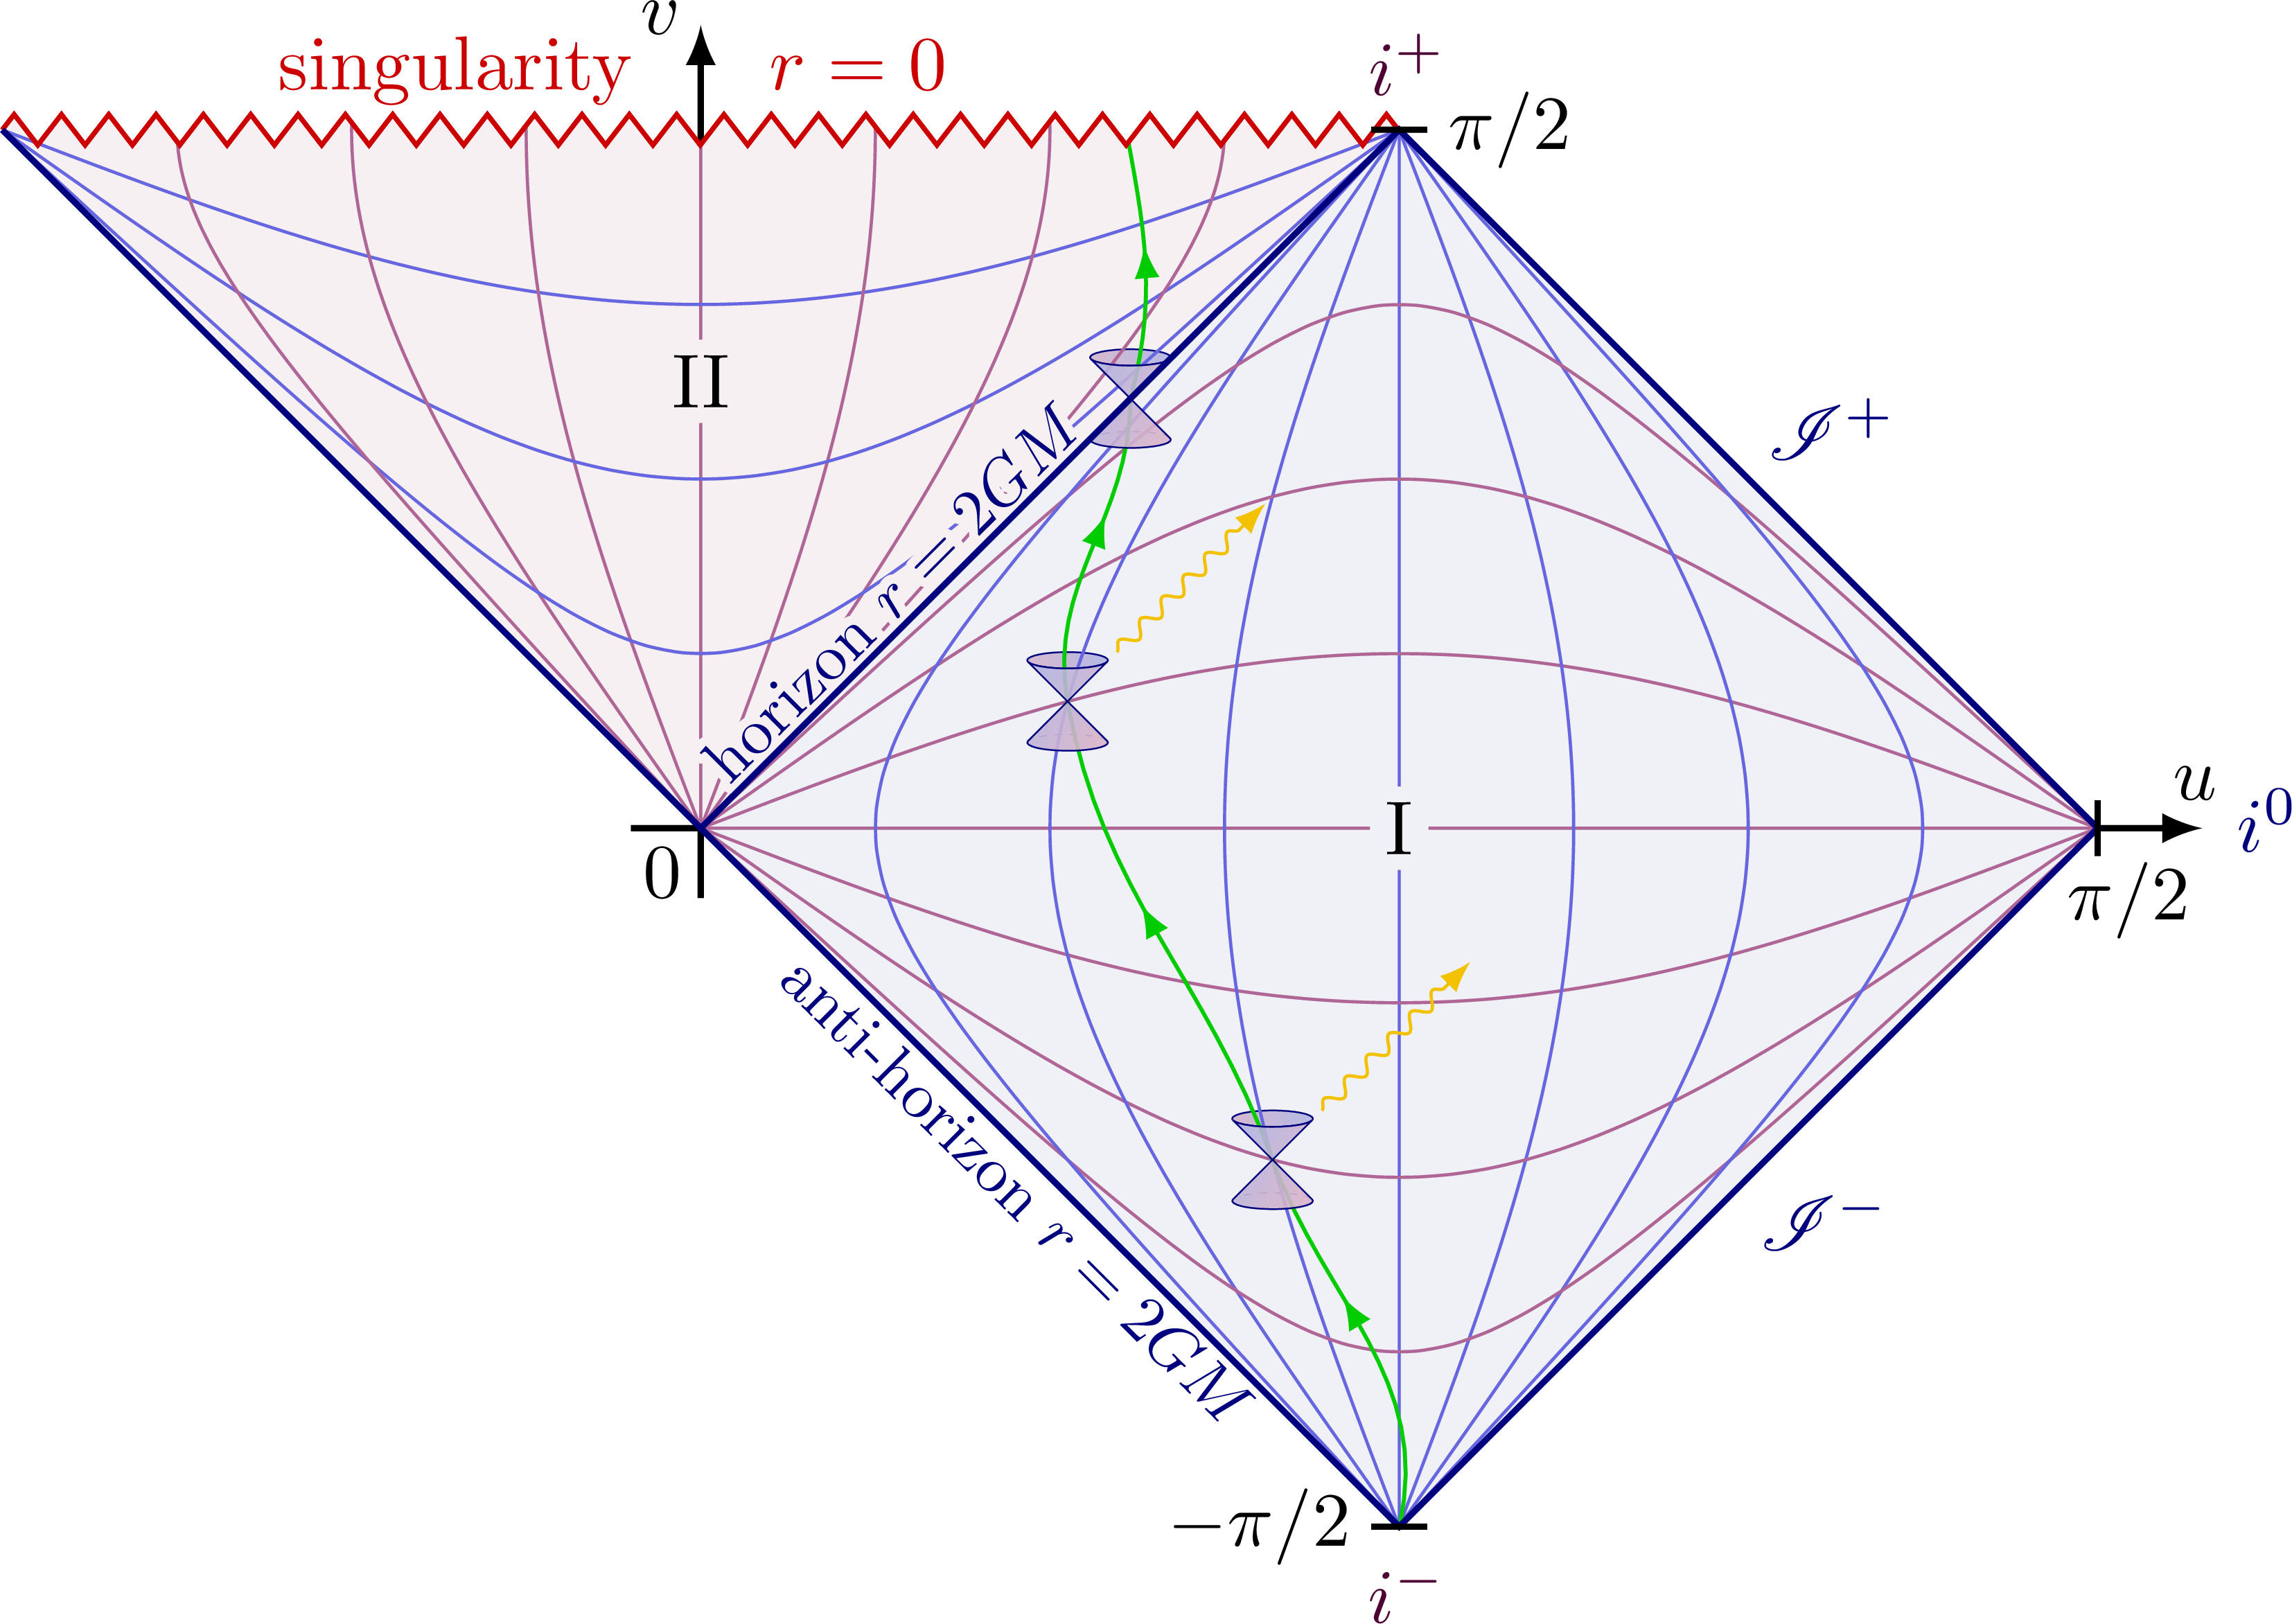
\includegraphics[alt={{Penrose diagram of the Schwarzschild blackhole solution}}, width=\linewidth]{images/schwarzschild_penrose_diagram.png}
\end{figure}
Zooming in on the singularity we can introduce two basis elements $\mathbf{B}_1$ and $\mathbf{B}_2$ of the Alexandrov topology one of which is ``$\varepsilon$ from the singularity'' and the second of which is ``$\varepsilon$ from $i^+$"
\begin{figure}[h]
    \centering
    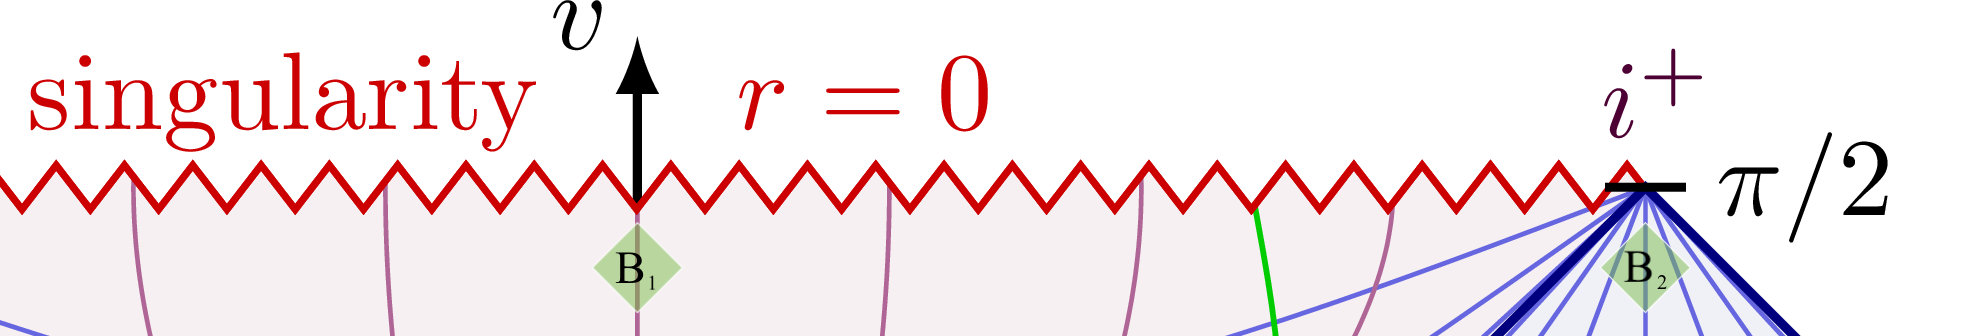
\includegraphics[alt={{Penrose diagram of the Schwarzschild blackhole solution zoomed to singularity and containing two basis elements}}, width=\linewidth]{images/schwarzschild_penrose_diagram_zoom1.png}
\end{figure}
What is obvious is that there exists no basis element $\mathbf{B}$ of the Alexandrov topology that contains both $\mathbf{B}_1$ and $\mathbf{B}_2$ as it would have to extend beyond the singularity off of $M_{BH}$ which is of course not allowed.

As a result of this, one can not employ the isotony axiom, the only tool one has, to place $\mathfrak{U}(\mathbf{B}_1)$ and $\mathfrak{U}(\mathbf{B}_2)$ in a larger algebra, an algebra in which addition and multiplication of their elements would make sense.

This implies that the set-theoretic union of all $\mathfrak{U}(\mathbf{B})$ over all basis elements $\mathbf{B}$ of the Alexandrov topology on $M_{BH}$ is not a normed *-algebra. This in turn implies that the construction of the quasilocal algebra fails\footnote{This argument can be formalized. However, doing so doesn't provide any insight beyond what's presented by this informal argument. Hence, we omitted the formal argument.} for $M_{BH}$.

For any two basis elements $\mathbf{B}_1$ and $\mathbf{B}_2$ of the Alexandrov topology on a generic Lorentzian spacetime $M$ the best one can hope for is that there exists a third element $\mathbf{B}$ of the Alexandrov topology such that $\mathbf{B}_1, \mathbf{B}_2 \subseteq \mathbf{B}$. However, there is no guarantee that such a $\mathbf{B}$ exists in a Lorentzian spacetime.

All that being said, we can still state a variation of Axiom 3 (Local Commutativity) that applies to a Lorentzian spacetime.

\subsection{Axiom 3 (Local Commutativity)}
The variation of Axiom 3 (Local Commutativity) as applied to Lorentzian spacetime is the following:

\begin{axiom}[Local Commutativity]
    Let $\mathbf{B}_1$ and $\mathbf{B}_2$ be any two basis elements of the Alexandrov topology on a Lorentzian spacetime, i.e. any two sets of the form $I^+(p_1) \cap I^-(q_1)$ and $I^+(p_2) \cap I^-(q_2)$.
    
    If $\mathbf{B_1}$ and $\mathbf{B_2}$ are completely spacelike, for any basis element $\mathbf{B}$ such that $\mathbf{B_1}, \mathbf{B_2} \subseteq \mathbf{B}$ the algebras $\mathfrak{U}(\mathbf{B_1})$ and $\mathfrak{U}(\mathbf{B_2})$ commute in the C*-algebra $\mathfrak{U}(\mathbf{B})$, i.e. for any $a_1$ in $\mathfrak{U}(\mathbf{B_1})$ and $a_2$ in $\mathfrak{U}(\mathbf{B_2})$ we have
    \begin{align}
        i(a_1) i(a_2) - i(a_2) i(a_1) = 0
    \end{align}
    in the C*-algebra $\mathfrak{U}(\mathbf{B})$, where $i$ is the unital *-monomorphism Axiom 2 (Isotony).
    
    If no such $\mathbf{B}$ exists, then it simply doesn't make sense to consider if $\mathfrak{U}(\mathbf{B_1})$ and $\mathfrak{U}(\mathbf{B_2})$ commute as they are not in the same algebra.
\end{axiom}

While having the commutation status of $\mathfrak{U}(\mathbf{B_1})$ and $\mathfrak{U}(\mathbf{B_2})$ sometimes being undefined seems ``odd'' at first. It's actually not ``odd'' at all. The commutation status of $\mathfrak{U}(\mathbf{B_1})$ and $\mathfrak{U}(\mathbf{B_2})$ is only undefined when it's impossible to conduct an experiment that determines if they commute. This makes complete sense.

\section{Axiom 4 (Local Algebra)}\label{sctn:axiom-4-(local-algebra)}
The axiom we are about to present also changes slightly from its analog Axiom 4 (Quasilocal Algebra) on Minkowski spacetime. The reason for the change, as was the reason for the change in Axiom 3 (Local Commutativity), is the fact that there is no such thing as a quasilocal algebra on a generic Lorentzian spacetime.

Before we state the next axiom for Lorentzian spacetimes, we need to, as in the case of Minkowski spacetime, present a definition used in the statement of the axiom.

This definition relies upon the fact, which one may check, that the GNS construction for a state $\omega$ on a C*-algebra $\mathfrak{U}(\mathbf{B})$, where $\mathbf{B}$ is an element of the Alexandrov topology on the Lorentzian spacetime $M$, works just as in the case of AQFT in Minkowski spacetime.

\begin{definition}[Local Observable]
    For Lorentzian spacetime $M$ the image $\pi_\omega(a)$ of a self-adjoint member $a$ of the local algebra $\mathfrak{U}(\mathbf{B})$ under the GNS *-homomorphism $\pi_\omega$ of a state $\omega$ on $\mathfrak{U}(\mathbf{B})$ is self-adjoint and thus corresponds to an ``observable''. Any ``observable'' corresponding to such a self-adjoint $\pi_\omega(a)$ is called a \textit{local observable}.
\end{local}

Using this definition we can state the axiom

\begin{axiom}[Local Algebra]
    All ``observables'' are local observables.
\end{axiom}

As shown in earlier in this blueprint, this axiom is essentially the statement that there exist ``observables'' that are not local observables, but such ``observables'' are ``experimentally indistinguishable'' from local observables and thus can be ignored.

\section{Axiom 5 (Isometric Covariance)}\label{sctn:axiom-5-(isometric-covariance)}
Now we present the final, and most interesting, axiom in the case of Lorentzian spacetimes.

The interesting aspect of this theorem is understanding what replaces the inhomogeneous Lorentz group connected to the identity, which appears in the Minkowski spacetime analog. One might think to replace it with diffeomorphisms of a Lorentzian spacetime. However, this isn't the correct analog.

Lorentzian spacetimes can admit diffeomorphisms that are not connected to the identity. (For example, in two dimensions \href{https://en.wikipedia.org/wiki/Dehn_twist}{Dehn twists} aren't connected to the identity.) So, if we want to ``mirror'' Axiom 5 (Lorentz Covariance) from the Minkowski case (which only considers group elements connected to the identity), we should limit the diffeomorphisms we employ.

So the ``natural'' choice seems to be the set of diffeomorphisms that are connected to the identity. However, this also isn't the correct analog.

Consider the case of Minkowski spacetime and the analogous axiom Axiom 5 (Lorentz Covariance). There the inhomogeneous Lorentz group connected to the identity is used. Under that group the Minkowski metric is invariant
\begin{align}
    \eta \longrightarrow \eta.
\end{align}
So instead of diffeomorphisms connected to the identity being used, what's being used here are isometries connected to the identity, i.e. diffeomorphism connected to the identity that leave the metric invariant.

So in the current case of a Lorentzian spacetime what we should be using are isometries connected to the identity. Using this, the axiom takes the following form:

\begin{axiom}[Isometric Covariance]
    Let $\mathbf{B}$ be any basis element of the Alexandrov topology on a Lorentzian spacetime $M$, i.e. any set of the form $I^+(p) \cap I^-(q)$.
    
    A member $\varphi$ of the group of isometries of $M$ connected to the identity acts on $\mathfrak{U}(\mathbf{B})$ as follows
    \begin{align}
        \alpha_\varphi : \mathfrak{U}(\mathbf{B}) &\longrightarrow \mathfrak{U}(\varphi(\mathbf{B})) \\
                                   a              &\longmapsto     \alpha_\varphi(a)
    \end{align}
    where $\varphi(\mathbf{B})$ is the image of the basis element $\mathbf{B}$ under the isometry $\varphi$ and $\alpha_\varphi$ is a unital *-isomorphism generated by $\varphi$. The map $\alpha_\varphi$ is such that (1) for the identity isometry $\mathbf{1}$ it satisfies
    \begin{align}
        \alpha_{\mathbf{1}}(a) = a,
    \end{align}
    (2) for all appropriate $a$, $\varphi$, and $\varphi'$ it satisfies
    \begin{align}
        \alpha_{\varphi' \cdot \varphi}(a) = \alpha_{\varphi'}(\alpha_{\varphi}(a)),
    \end{align}
    and (3) for basis elements $\mathbf{B}_\iota \subset \mathbf{B}_\kappa$ and the unital *-monomorphism $i$ of Axiom 2 (Isotony) $\alpha_\varphi$ commutes with $i$. In other words the following diagram

    \begin{center}
        \begin{tikzcd}
            \mathfrak{U}(\mathbf{B}_\kappa) \arrow[r, "\alpha_\varphi"]
            & \mathfrak{U}(\varphi(\mathbf{B}_\kappa)) \\
            \mathfrak{U}(\mathbf{B}_\iota) \arrow[r, "\alpha_\varphi"]  \arrow[u, "i"]
            & \mathfrak{U}(\varphi(\mathbf{B}_\iota))  \arrow[u, "i"]
        \end{tikzcd}
    \end{center}

    commutes.
\end{axiom}


\section{Haag Kastler Axioms in Curved Spacetime}\label{sctn:haag-kastler-axioms-in-curved-spacetime}
Here we recount the axioms we've established for AQFT in Lorentzian spacetime.

The first axiom states:

\begin{definition}[Axiom 1: Local Algebras]
    \label{def:local-algebras-in-curved-spacetime}
    \uses{def:alexandrov-topology}
    \uses{def:lorentzian-spacetime}
    \uses{def:chronological-future-and-chronological-past}
    For any basis element $\mathbf{B}$ of the Alexandrov topology on a Lorentzian spacetime, i.e. any set of the form $I^+(p) \cap I^-(q)$, there is a corresponding abstract C*-algebra $\mathfrak{U}(\mathbf{B})$
    \begin{align}
        \mathbf{B} \longmapsto \mathfrak{U}(\mathbf{B}),
    \end{align}
    and when $\mathbf{B}$ is the empty set, we have the distinguished correspondence
    \begin{align}
        \emptyset \longmapsto \mathbb{C} \mathbf{1},
    \end{align}
    where $\mathbf{1}$ is the multiplicative identity in the abstract C*-algebra $\mathbb{C} \mathbf{1}$.
\end{definition}

The second axiom can be immediately stated too.

\begin{definition}[Axiom 2: Isotony]
    \label{def:isotony-in-curved-spacetime}
    \uses{def:alexandrov-topology}
    \uses{def:lorentzian-spacetime}
    \uses{def:chronological-future-and-chronological-past}
    \uses{def:local-algebras-in-curved-spacetime}
    Let $\mathbf{B}_1$ and $\mathbf{B}_2$ be any two basis elements of the Alexandrov topology on a Lorentzian spacetime, i.e. any two sets of the form $I^+(p_1) \cap I^-(q_1)$ and $I^+(p_2) \cap I^-(q_2)$.
    
    If $\mathbf{B}_1 \subset \mathbf{B}_2$ then $\mathfrak{U}(\mathbf{B}_1) \subset \mathfrak{U}(\mathbf{B}_2)$, where inclusion is implemented by
    \begin{align}
        i : \mathfrak{U}(\mathbf{B}_1) \hookrightarrow \mathfrak{U}(\mathbf{B}_2),
    \end{align}
    a unital *-monomorphism.
\end{definition}

The next axiom can be stated as follows:

\begin{definition}[Axiom 3: Local Commutativity]
    \label{def:local-commutativity-in-curved-spacetime}
    \uses{def:alexandrov-topology}
    \uses{def:lorentzian-spacetime}
    \uses{def:chronological-future-and-chronological-past}
    \uses{def:completely-spacelike}
    \uses{def:local-algebras-in-curved-spacetime} 
    Let $\mathbf{B}_1$ and $\mathbf{B}_2$ be any two basis elements of the Alexandrov topology on a Lorentzian spacetime, i.e. any two sets of the form $I^+(p_1) \cap I^-(q_1)$ and $I^+(p_2) \cap I^-(q_2)$.
    
    If $\mathbf{B_1}$ and $\mathbf{B_2}$ are completely spacelike, for any Alexandrov topology basis element $\mathbf{B}$ such that $\mathbf{B_1}, \mathbf{B_2} \subseteq \mathbf{B}$ the algebras $\mathfrak{U}(\mathbf{B_1})$ and $\mathfrak{U}(\mathbf{B_2})$ commute in the C*-algebra $\mathfrak{U}(\mathbf{B})$, i.e. for any $a_1$ in $\mathfrak{U}(\mathbf{B_1})$ and $a_2$ in $\mathfrak{U}(\mathbf{B_2})$ we have
    \begin{align}
        i(a_1) i(a_2) - i(a_2) i(a_1) = 0
    \end{align}
    in the C*-algebra $\mathfrak{U}(\mathbf{B})$, where $i$ is the unital *-monomorphism Axiom 2 (Isotony).
    
    If no such $\mathbf{B}$ exists, then it simply doesn't make sense to consider if $\mathfrak{U}(\mathbf{B_1})$ and $\mathfrak{U}(\mathbf{B_2})$ commute as they are not in the same algebra.
\end{definition}

The next axiom has need of the following definition

\begin{definition}[Local Observable]
    \label{def:local-observable}
    \uses{def:lorentzian-spacetime}
    \uses{thrm:gns-construction-theorem}
    \uses{def:local-algebras-in-curved-spacetime} 
    \uses{def:state}
    For Lorentzian spacetime $M$ the image $\pi_\omega(a)$ of a self-adjoint member $a$ of the local algebra $\mathfrak{U}(\mathbf{B})$ under the GNS *-homomorphism $\pi_\omega$ of a state $\omega$ on $\mathfrak{U}(\mathbf{B})$ is self-adjoint and thus corresponds to an ``observable''. Any ``observable'' corresponding to such a self-adjoint $\pi_\omega(a)$ is called a \textit{local observable}.
\end{definition}

and can be stated as follows:

\begin{definition}[Axiom 4: Local Completeness]
    \label{def:local-completeness-in-curved-spacetime}
    \uses{def:local-observable}
    All ``observables'' are local observables.
\end{definition}

The final axiom states:

\begin{definition}[Axiom 5: Isometric Covariance]
    \label{def:isometric-covariance-in-curved-spacetime}
    \uses{def:alexandrov-topology}
    \uses{def:lorentzian-spacetime}
    \uses{def:chronological-future-and-chronological-past}
    \uses{def:local-algebras-covariance-in-curved-spacetime}
    \uses{def:isotony-covariance-in-curved-spacetime}
    Let $\mathbf{B}$ be any basis element of the Alexandrov topology on a Lorentzian spacetime $M$, i.e. any set of the form $I^+(p) \cap I^-(q)$.
    
    A member $\varphi$ of the group of isometries of $M$ connected to the identity acts on $\mathfrak{U}(\mathbf{B})$ as follows
    \begin{align}
        \alpha_\varphi : \mathfrak{U}(\mathbf{B}) &\longrightarrow \mathfrak{U}(\varphi(\mathbf{B})) \\
                                   a              &\longmapsto     \alpha_\varphi(a)
    \end{align}
    where $\varphi(\mathbf{B})$ is the image of the basis element $\mathbf{B}$ under the isometry $\varphi$ and $\alpha_\varphi$ is a unital *-isomorphism generated by $\varphi$. The map $\alpha_\varphi$ is such that (1) for the identity isometry $\mathbf{1}$ it satisfies
    \begin{align}
        \alpha_{\mathbf{1}}(a) = a,
    \end{align}
    (2) for all appropriate $a$, $\varphi$, and $\varphi'$ it satisfies
    \begin{align}
        \alpha_{\varphi' \circ \varphi}(a) = \alpha_{\varphi'}(\alpha_{\varphi}(a)),
    \end{align}
    and (3) for Alexandrov topology basis elements $\mathbf{B}_\iota \subset \mathbf{B}_\kappa$ and the unital *-monomorphism $i$ of Axiom 2 (Isotony) $\alpha_\varphi$ commutes with $i$. In other words the following diagram

    \begin{center}
        \begin{tikzcd}
            \mathfrak{U}(\mathbf{B}_\kappa) \arrow[r, "\alpha_\varphi"]
            & \mathfrak{U}(\varphi(\mathbf{B}_\kappa)) \\
            \mathfrak{U}(\mathbf{B}_\iota) \arrow[r, "\alpha_\varphi"]  \arrow[u, "i"]
            & \mathfrak{U}(\varphi(\mathbf{B}_\iota))  \arrow[u, "i"]
        \end{tikzcd}
    \end{center}

    commutes.
\end{definition}

Generally these axioms follow in a straightforward manner from those of AQFT in Minkowski spacetime. The only ``surprise'' in this presentation is the absence of a quasilocal algebra. However, as we found, its absence is simply a reflection of the observational constraints of Lorentzian spacetime which don't exist in Minkowski spacetime.
